\newpage

\chapter{Théorie naïve des ensembles}
\vspace{4mm} %5mm vertical space

\section{Définition}

on appelle ensemble, une collection d'objets appellés éléments de cet ensemble.\\
un objet particulier appartient ($\in$) ou n'appartient pas ($\notin$) à un ensemble donné.\\

Exemple d'ensemble : l'ensemble des voyelles : V=\{a,e,i,o,u,y\} \\

a $\in$ V : a appartient à l'ensemble V \\
d $\notin$ V : d n'appartient pas à l'ensemble V \\

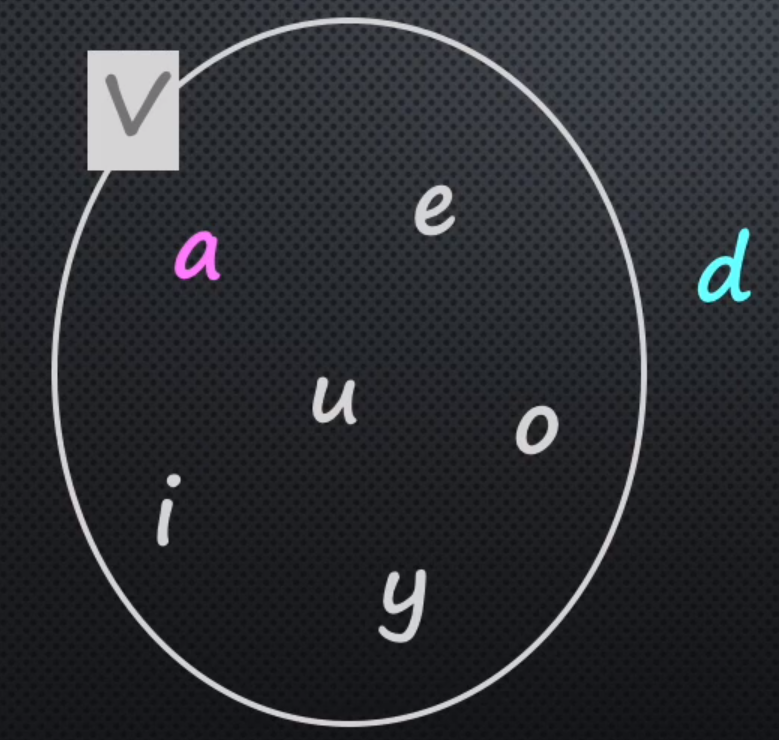
\includegraphics[scale=0.2]{Ensembles}
\vspace{3mm} %5mm vertical space

\section{Relation d'inclusion}

Soient A et B sont deux ensembles, on dit que A est inclus dans B (Noté A$\subset$ B), si tout les éléments de A sont des éléments de B.
Autrement dit (X$\subset$A) et que (X$\subset$B).\\

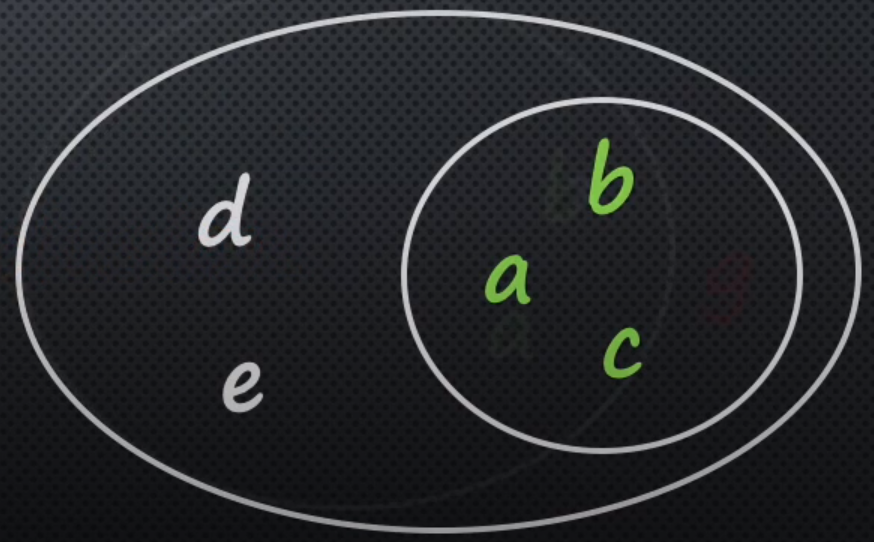
\includegraphics[scale=0.2]{EnsemblesInc}
\vspace{3mm} %5mm vertical space

On peut dire que \{a,b,g\}$\in$\{a,b,d,e\} \\

\section{Propriété de l'inclusion}

\begin{itemize}
\item {a. Reflexivité : pour tout ensemble A (A$\in$B)}
\item {b. Anti-Symétrique : (A$\in$B) et (B$\in$A) $=>$ A=B}
\item {c. Transitivité : (A$\in$B) et (B$\in$C) $=>$ (A$\in$C)}
\end{itemize}

\newpage
\section{Relation d'égalité}

Soient A et B sont deux ensembles, on dit que A égale B (Noté A=B), si tout les éléments de A appartient à B. Autrement dit (X$\in$A) et que (X$\in$B).

\section{Opération d'union ($\cup$)}
\vspace{3mm} %5mm vertical space

1) L'union de 2 ensembles \\

A= \{a,e\} et B = \{b,c,d\} \\

C = A $\cup$ B = \{a,e,b,c,d\}

\vspace{3mm} %5mm vertical space
\section{Opération d'intersection ($\cap$)}
\vspace{3mm} %5mm vertical space

\textbf{Intersection de 2 ensembles} \\

Soient A et B deux ensembles, on appelle (A$\cap$B) le nouvel ensemble contenant les éléments se trouvant dans A et B. \\

A= \{a,b\} et B = \{b,c,d\} \\

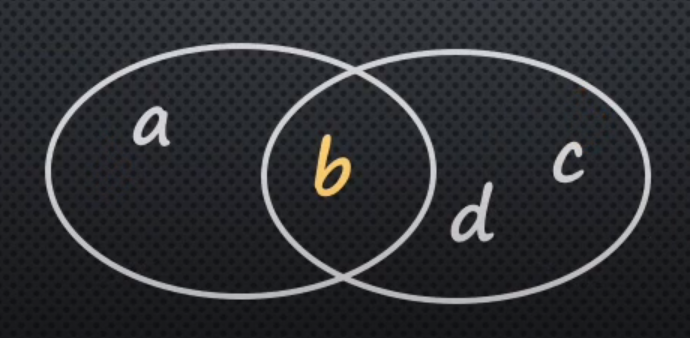
\includegraphics[scale=0.2]{EnsemblesInt}
\vspace{3mm} %5mm vertical space

C = A $\cap$ B = \{b\} \\

\section{Ensemble vide}

L'ensemble vide est une partie (un sous-ensemble) de n'importe quel ensembles.\\
Il ne possède qu'un seul sous-ensemble : lui-même \\

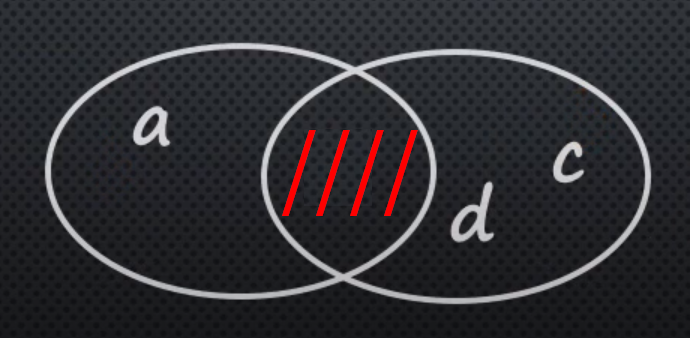
\includegraphics[scale=0.2]{EnsemblesVide}
\vspace{3mm} %5mm vertical space

C = A $\cap$ B = \{$\oslash$\}

\newpage
\section{Cardinalité}

Soit A un ensemble, Si A possède exactement N éléments (n $\in$ \N), A est un ensemble fini de cardinalité N.\\

Noté $|A|$ = n \\

$|1,2,3|$ = 3 \\

$|\oslash|$ = 0 \\

$|\{\oslash\}|$ = 1 \\

$|P(A)|$ = 2$^{k}$ ou K est le nombre d'éléments dans A \\

P(A) est l'ensemble des parties \\

\section{Identité}

A $\cup$ A = A \\
A $\cap$ A = A \\

\section{Commutativité}

A $\cap$ B  = B $\cap$ A \\
A $\cup$ B  = B $\cup$ A \\

\section{Associativité}

A $\cap$ (B $\cap$ C) = (A $\cap$ B) $\cap$ C \\
A $\cup$ (B $\cup$ C) = (A $\cup$ B) $\cup$ C \\

\section{Distributivité}

A $\cap$ (B $\cup$ C) = (A $\cap$ B) $\cup$ (A $\cap$ C) \\
A $\cup$ (B $\cap$ C) = (A $\cup$ B) $\cap$ (A $\cup$ C) \\

\section{De Morgans}

¬(A $\cup$ B) = ¬A $\cap$ ¬B) \\
¬(A $\cap$ B) = ¬A $\cup$ ¬B) \\
